\chapter{Specification - (SRS)}

\section{Introduction}
\subsection{Purpose of this document}
The purpose of this document is to define the requirements to be met by the system to be classified as successful and functional.

\subsection{Scope of this document}
The system is wholly engineered and developed by me, with the supervision of Dr. Wael Gomaa. The users are the professors of MSA University's Faculty of Languages.

\subsection{Overview}
The system will take a collection of texts, organized by author, to be analyzed by the system through a set of stylometric and linguistic features, and will return the extracted features embedded in the text with a statistical report of the analysis. The system will also require a selection of predefined grammar sets defined by the user and/or the community.

\subsection{Business Context}
The MSA University Faculty of Languages is the organization supporting and contributing to the project.

\section{General Description}
\subsection{Product Functions}
\begin{enumerate}
    \item Create new project.
    \item Upload texts.
    \item Select from predefined grammar sets.
    \item Create new grammar sets.
    \item Extract stylistic and linguistic features.
    \item Statistical analysis.
    \item Highlight the extracted features.
    \item Modify analysis results.
    \item Login
    \item Logout
    \item Signup
\end{enumerate}
\subsection{User Characteristics}
The users will be linguistic professionals that can verify the output of the system, and are able to evaluate and verify the results of the analysis.
\subsection{User Problem Statement}
The main problem the system is facing is the time consuming labor involved in extracting those linguistic features and their analysis.
\subsection{User Objectives}
\begin{itemize}
    \item Identify features of the text.
    \item Modify the analysis results.
    \item Identify the disputed text's author.
    \item Create custom grammar for new features.
\end{itemize}

\section{Functional Requirements}
\begin{center}
    \begin{table}[H]
        \caption{Create New Project}
        \begin{tabularx}{\textwidth} {
                | >{\raggedright\arraybackslash\hsize=.5\hsize\linewidth=\hsize}X
                | >{\raggedright\arraybackslash\hsize=1.5\hsize\linewidth=\hsize}X |}
            \hline
            Function Name                        & Create New Project                                                                                  \\ \hline
            Description                          & The user will create a new project that will host the documents of the same context to be analyzed. \\ \hline
            Critical                             & This requirement is the opening point of the system, so the system cannot work without it.          \\ \hline
            Technical issues                     & None.                                                                                               \\ \hline
            Risks                                & None.                                                                                               \\ \hline
            Dependencies with other requirements & None.                                                                                               \\ \hline
            Precondition                         & Starting state.                                                                                     \\ \hline
            Post-Condition                       & Awaiting documents to be uploaded.                                                                  \\ \hline
        \end{tabularx}
    \end{table}
\end{center}

\begin{center}
    \begin{table}[H]
        \caption{Upload Texts}
        \begin{tabularx}{\textwidth} {
                | >{\raggedright\arraybackslash\hsize=.5\hsize\linewidth=\hsize}X
                | >{\raggedright\arraybackslash\hsize=1.5\hsize\linewidth=\hsize}X |}
            \hline
            Function Name                        & Upload Texts                                                                                                                                                                                \\ \hline
            Description                          & The user will upload a collection of texts with each group of texts put in a separate folder with the label of the folder being the name of the author, and the disputed text if available. \\ \hline
            Critical                             & This requirement is the opening point of the project, so the system cannot work without it.                                                                                                 \\ \hline
            Technical issues                     & Detecting the user uploaded the texts in the proper format.                                                                                                                                 \\ \hline
            Risks                                & None.                                                                                                                                                                                       \\ \hline
            Dependencies with other requirements & 'Create New Project'                                                                                                                                                                        \\ \hline
            Precondition                         & A new project is created.                                                                                                                                                                   \\ \hline
            Post-Condition                       & Awaiting the features to be explored.                                                                                                                                                       \\ \hline
        \end{tabularx}
    \end{table}
\end{center}

\begin{center}
    \begin{table}[H]
        \caption{Select from predefined grammar sets}
        \begin{tabularx}{\textwidth} {
                | >{\raggedright\arraybackslash\hsize=.5\hsize\linewidth=\hsize}X
                | >{\raggedright\arraybackslash\hsize=1.5\hsize\linewidth=\hsize}X |}
            \hline
            Function Name                        & Select from predefined grammar sets                                               \\ \hline
            Description                          & The user will select a number of grammar sets that the text will be analyzed for. \\ \hline
            Critical                             & System can't advance without it.                                                  \\ \hline
            Technical issues                     & None.                                                                             \\ \hline
            Risks                                & None.                                                                             \\ \hline
            Dependencies with other requirements & None.                                                                             \\ \hline
            Precondition                         & Texts have been uploaded.                                                         \\ \hline
            Post-Condition                       & Awaiting analysis results.                                                        \\ \hline
        \end{tabularx}
    \end{table}
\end{center}

\begin{center}
    \begin{table}[H]
        \caption{Create new grammar sets}
        \begin{tabularx}{\textwidth} {
                | >{\raggedright\arraybackslash\hsize=.5\hsize\linewidth=\hsize}X
                | >{\raggedright\arraybackslash\hsize=1.5\hsize\linewidth=\hsize}X |}
            \hline
            Function Name                        & Create new grammar sets                                                                                                                                                               \\ \hline
            Description                          & The user will be presented with an interface that will allow them to define their own grammar to apply on the corpus. The generated grammar will also be saved to the user's account. \\ \hline
            Critical                             & Optional.                                                                                                                                                                             \\ \hline
            Technical issues                     & Ensuring that the grammar is of proper and valid format.                                                                                                                              \\ \hline
            Risks                                & None.                                                                                                                                                                                 \\ \hline
            Dependencies with other requirements & None.                                                                                                                                                                                 \\ \hline
            Precondition                         & Grammar sets have been selected.                                                                                                                                                      \\ \hline
            Post-Condition                       & Awaiting analysis of the corpus.                                                                                                                                                      \\ \hline
        \end{tabularx}
    \end{table}
\end{center}

\begin{center}
    \begin{table}[H]
        \caption{Extract stylistic and linguistic features}
        \begin{tabularx}{\textwidth} {
                | >{\raggedright\arraybackslash\hsize=.5\hsize\linewidth=\hsize}X
                | >{\raggedright\arraybackslash\hsize=1.5\hsize\linewidth=\hsize}X |}
            \hline
            Function Name                        & Extract stylistic and linguistic features                                                                 \\ \hline
            Description                          & The system will receive the user's input and proceed to make the required analysis and return the result. \\ \hline
            Critical                             & Critical, system can't function without it.                                                               \\ \hline
            Technical issues                     & None.                                                                                                     \\ \hline
            Risks                                & None.                                                                                                     \\ \hline
            Dependencies with other requirements & 'Create New Project', and 'Upload texts', 'Select from predefined grammar sets'                           \\ \hline
            Precondition                         & Grammar is selected.                                                                                      \\ \hline
            Post-Condition                       & Feature extraction is complete and returned to the user.                                                  \\ \hline
        \end{tabularx}
    \end{table}
\end{center}

\begin{center}
    \begin{table}[H]
        \caption{Statistical analysis}
        \begin{tabularx}{\textwidth} {
                | >{\raggedright\arraybackslash\hsize=.5\hsize\linewidth=\hsize}X
                | >{\raggedright\arraybackslash\hsize=1.5\hsize\linewidth=\hsize}X |}
            \hline
            Function Name                        & Statistical analysis.                                                                          \\ \hline
            Description                          & The system will apply statistical analysis to the extracted features received from the parser. \\ \hline
            Critical                             & Critical, system can't function without it.                                                    \\ \hline
            Technical issues                     & None.                                                                                          \\ \hline
            Risks                                & None.                                                                                          \\ \hline
            Dependencies with other requirements & 'Extract stylistic and linguistic features'                                                    \\ \hline
            Precondition                         & Features are extracted.                                                                        \\ \hline
            Post-Condition                       & Statistical analysis is applied and ready for modification.                                    \\ \hline
        \end{tabularx}
    \end{table}
\end{center}

\begin{center}
    \begin{table}[H]
        \caption{Highlight the extracted features}
        \begin{tabularx}{\textwidth} {
                | >{\raggedright\arraybackslash\hsize=.5\hsize\linewidth=\hsize}X
                | >{\raggedright\arraybackslash\hsize=1.5\hsize\linewidth=\hsize}X |}
            \hline
            Function Name                        & Highlight the extracted features.                                                                                                      \\ \hline
            Description                          & The system will highlight the extracted features in the work space section of the project and offer methods of editing of the results. \\ \hline
            Critical                             & Not critical.                                                                                                                          \\ \hline
            Technical issues                     & None.                                                                                                                                  \\ \hline
            Risks                                & None.                                                                                                                                  \\ \hline
            Dependencies with other requirements & 'Extract stylistic and linguistic features'                                                                                            \\ \hline
            Precondition                         & Features are extracted.                                                                                                                \\ \hline
            Post-Condition                       & System awaiting features modification.                                                                                                 \\ \hline
        \end{tabularx}
    \end{table}
\end{center}

\begin{center}
    \begin{table}[H]
        \caption{Modify analysis results}
        \begin{tabularx}{\textwidth} {
                | >{\raggedright\arraybackslash\hsize=.5\hsize\linewidth=\hsize}X
                | >{\raggedright\arraybackslash\hsize=1.5\hsize\linewidth=\hsize}X |}
            \hline
            Function Name                        & Modify analysis results.                                                                                \\ \hline
            Description                          & The user can hover over a word in the work space (highlighted or not) and edit its feature association. \\ \hline
            Critical                             & Not critical.                                                                                           \\ \hline
            Technical issues                     & None.                                                                                                   \\ \hline
            Risks                                & None.                                                                                                   \\ \hline
            Dependencies with other requirements & 'Highlight extracted features'                                                                          \\ \hline
            Precondition                         & Features are highlighted in the work space.                                                             \\ \hline
            Post-Condition                       & Modifications are applied to the work space and the statistical analysis.                               \\ \hline
        \end{tabularx}
    \end{table}
\end{center}

\begin{center}
    \begin{table}[H]
        \caption{Login}
        \begin{tabularx}{\textwidth} {
                | >{\raggedright\arraybackslash\hsize=.5\hsize\linewidth=\hsize}X
                | >{\raggedright\arraybackslash\hsize=1.5\hsize\linewidth=\hsize}X |}
            \hline
            Function Name                        & Login.                                               \\ \hline
            Description                          & User is logged in to system using their credentials. \\ \hline
            Critical                             & Critical.                                            \\ \hline
            Technical issues                     & None.                                                \\ \hline
            Risks                                & None.                                                \\ \hline
            Dependencies with other requirements & None.                                                \\ \hline
            Precondition                         & User has no access to the system.                    \\ \hline
            Post-Condition                       & User is greeted with the home screen.                \\ \hline
        \end{tabularx}
    \end{table}
\end{center}

\begin{center}
    \begin{table}[H]
        \caption{Logout}
        \begin{tabularx}{\textwidth} {
                | >{\raggedright\arraybackslash\hsize=.5\hsize\linewidth=\hsize}X
                | >{\raggedright\arraybackslash\hsize=1.5\hsize\linewidth=\hsize}X |}
            \hline
            Function Name                        & Logout.                                                            \\ \hline
            Description                          & User is logged out of the system and is greeted with the homepage. \\ \hline
            Critical                             & Critical.                                                          \\ \hline
            Technical issues                     & None.                                                              \\ \hline
            Risks                                & None.                                                              \\ \hline
            Dependencies with other requirements & None.                                                              \\ \hline
            Precondition                         & User has access to the system.                                     \\ \hline
            Post-Condition                       & User is greeted with the Login screen.                             \\ \hline
        \end{tabularx}
    \end{table}
\end{center}

\begin{center}
    \begin{table}[H]
        \caption{Sign-up}
        \begin{tabularx}{\textwidth} {
                | >{\raggedright\arraybackslash\hsize=.5\hsize\linewidth=\hsize}X
                | >{\raggedright\arraybackslash\hsize=1.5\hsize\linewidth=\hsize}X |}
            \hline
            Function Name                        & Sign-up.                                                                    \\ \hline
            Description                          & User creates a new account using their credentials.                         \\ \hline
            Critical                             & Critical.                                                                   \\ \hline
            Technical issues                     & None.                                                                       \\ \hline
            Risks                                & None.                                                                       \\ \hline
            Dependencies with other requirements & None.                                                                       \\ \hline
            Precondition                         & User has no account registered in the system.                               \\ \hline
            Post-Condition                       & User account is registered and they are greeted with the system's homepage. \\ \hline
        \end{tabularx}
    \end{table}
\end{center}

\section{Interface Requirements}
\subsection{User Interfaces}
\subsubsection {GUI}
\begin{figure}[H]
    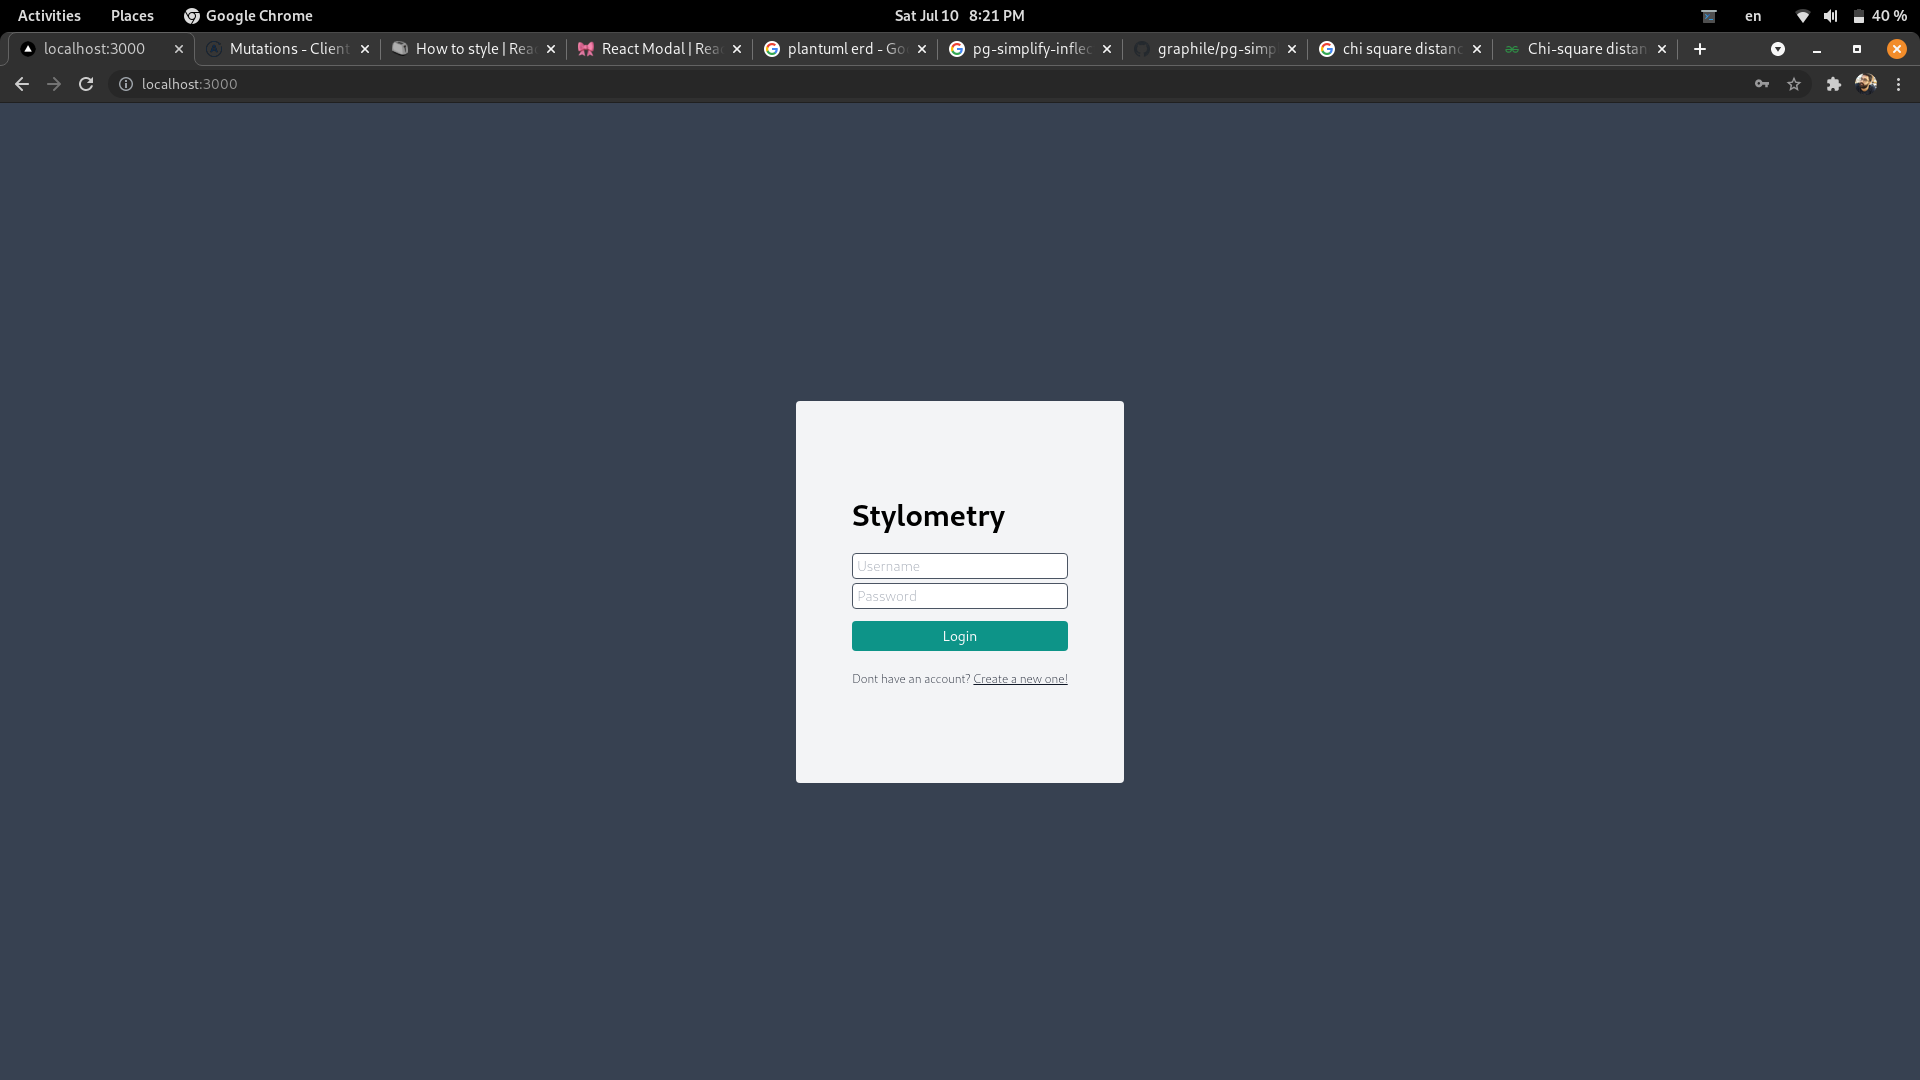
\includegraphics[width=15cm]{images/Login.png}
    \caption{Login}
\end{figure}

\begin{figure}[H]
    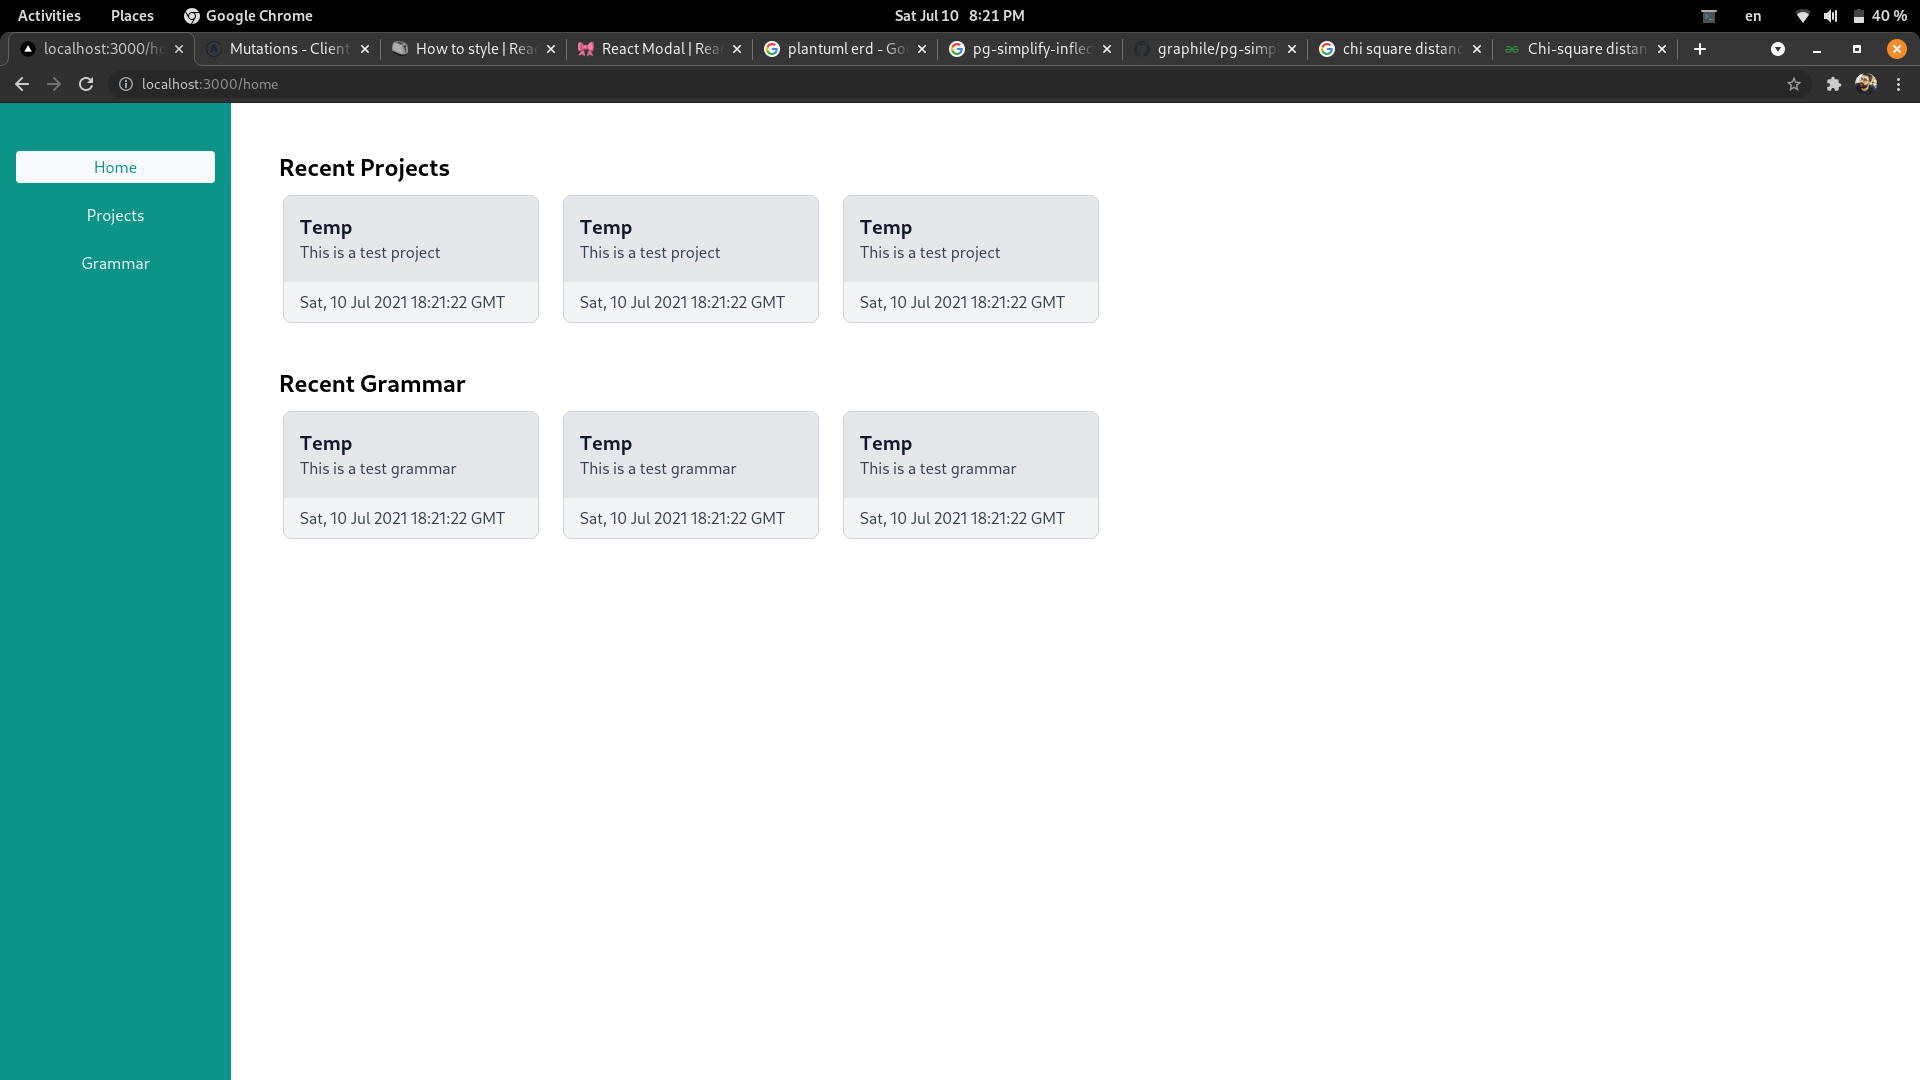
\includegraphics[width=15cm]{images/Home.png}
    \caption{Home}
\end{figure}

\begin{figure}[H]
    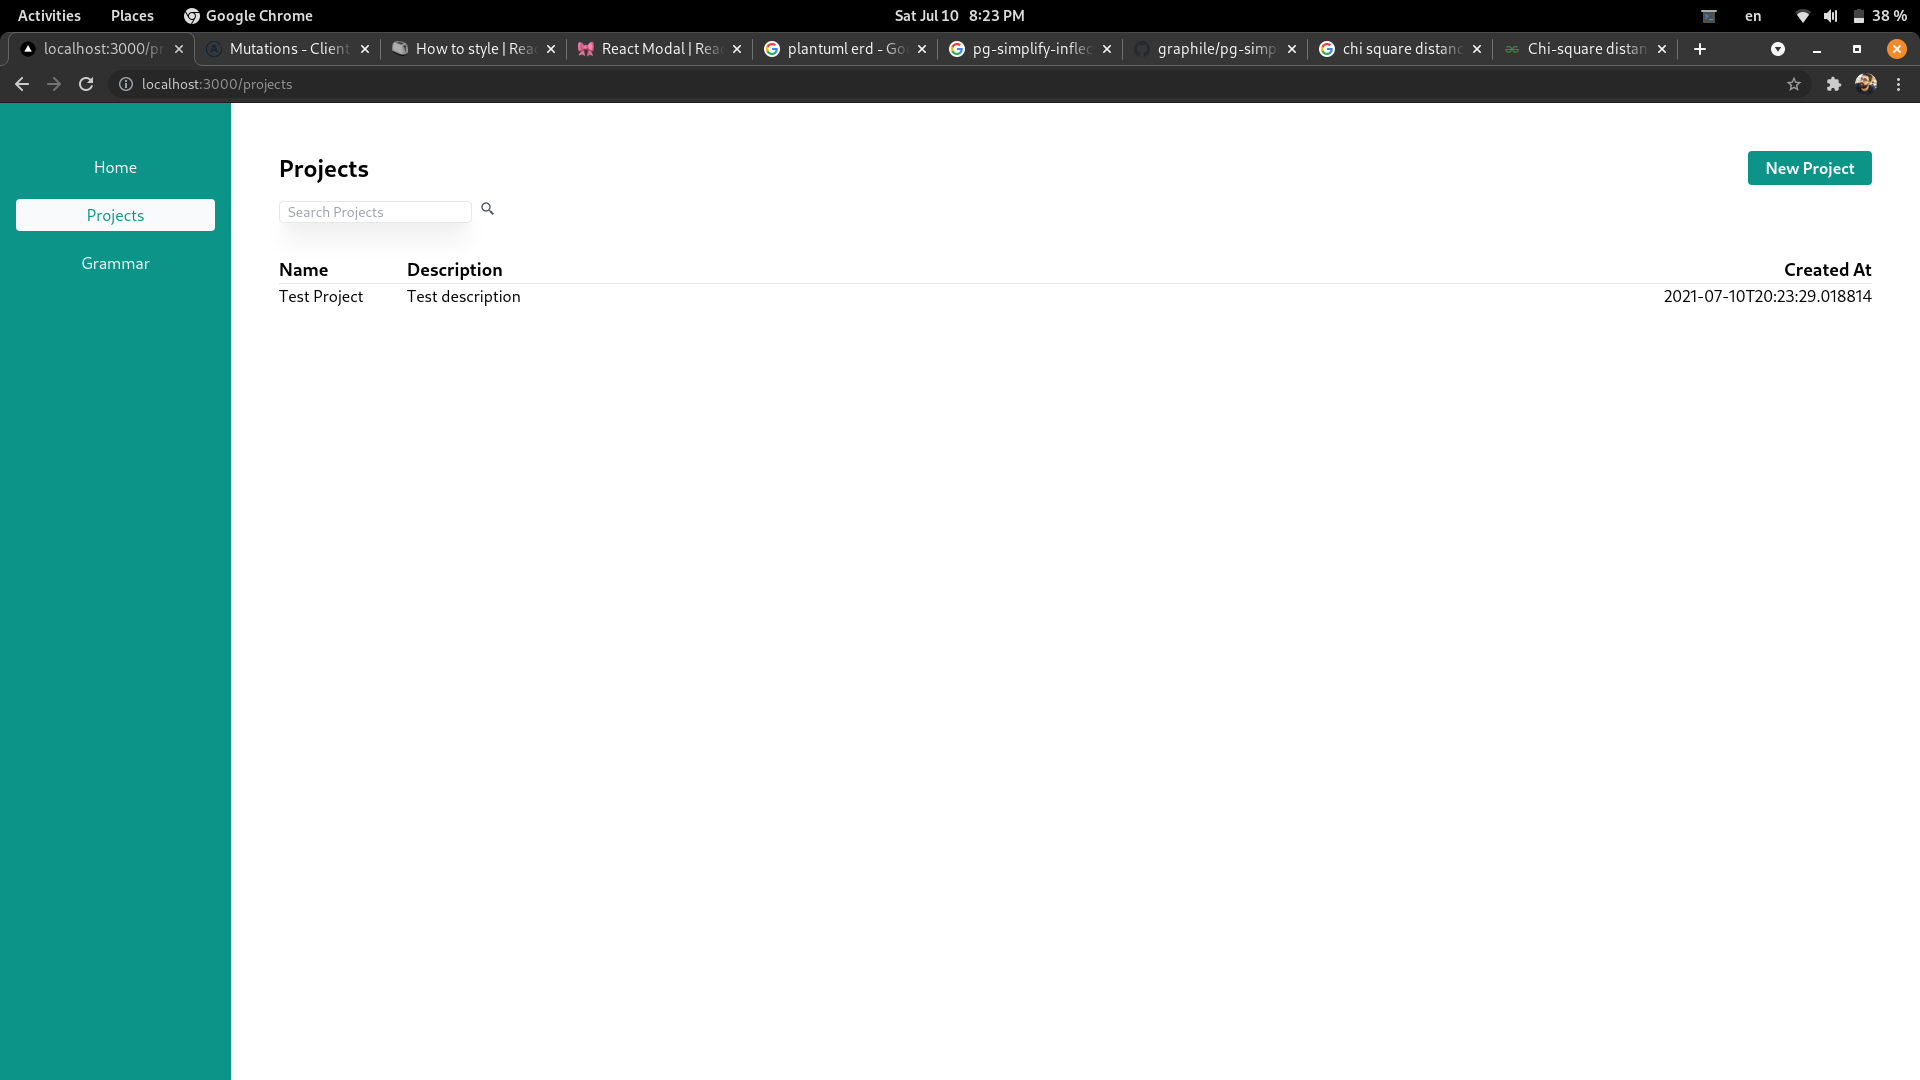
\includegraphics[width=15cm]{images/Projects.png}
    \caption{Projects}
\end{figure}
\begin{figure}[H]
    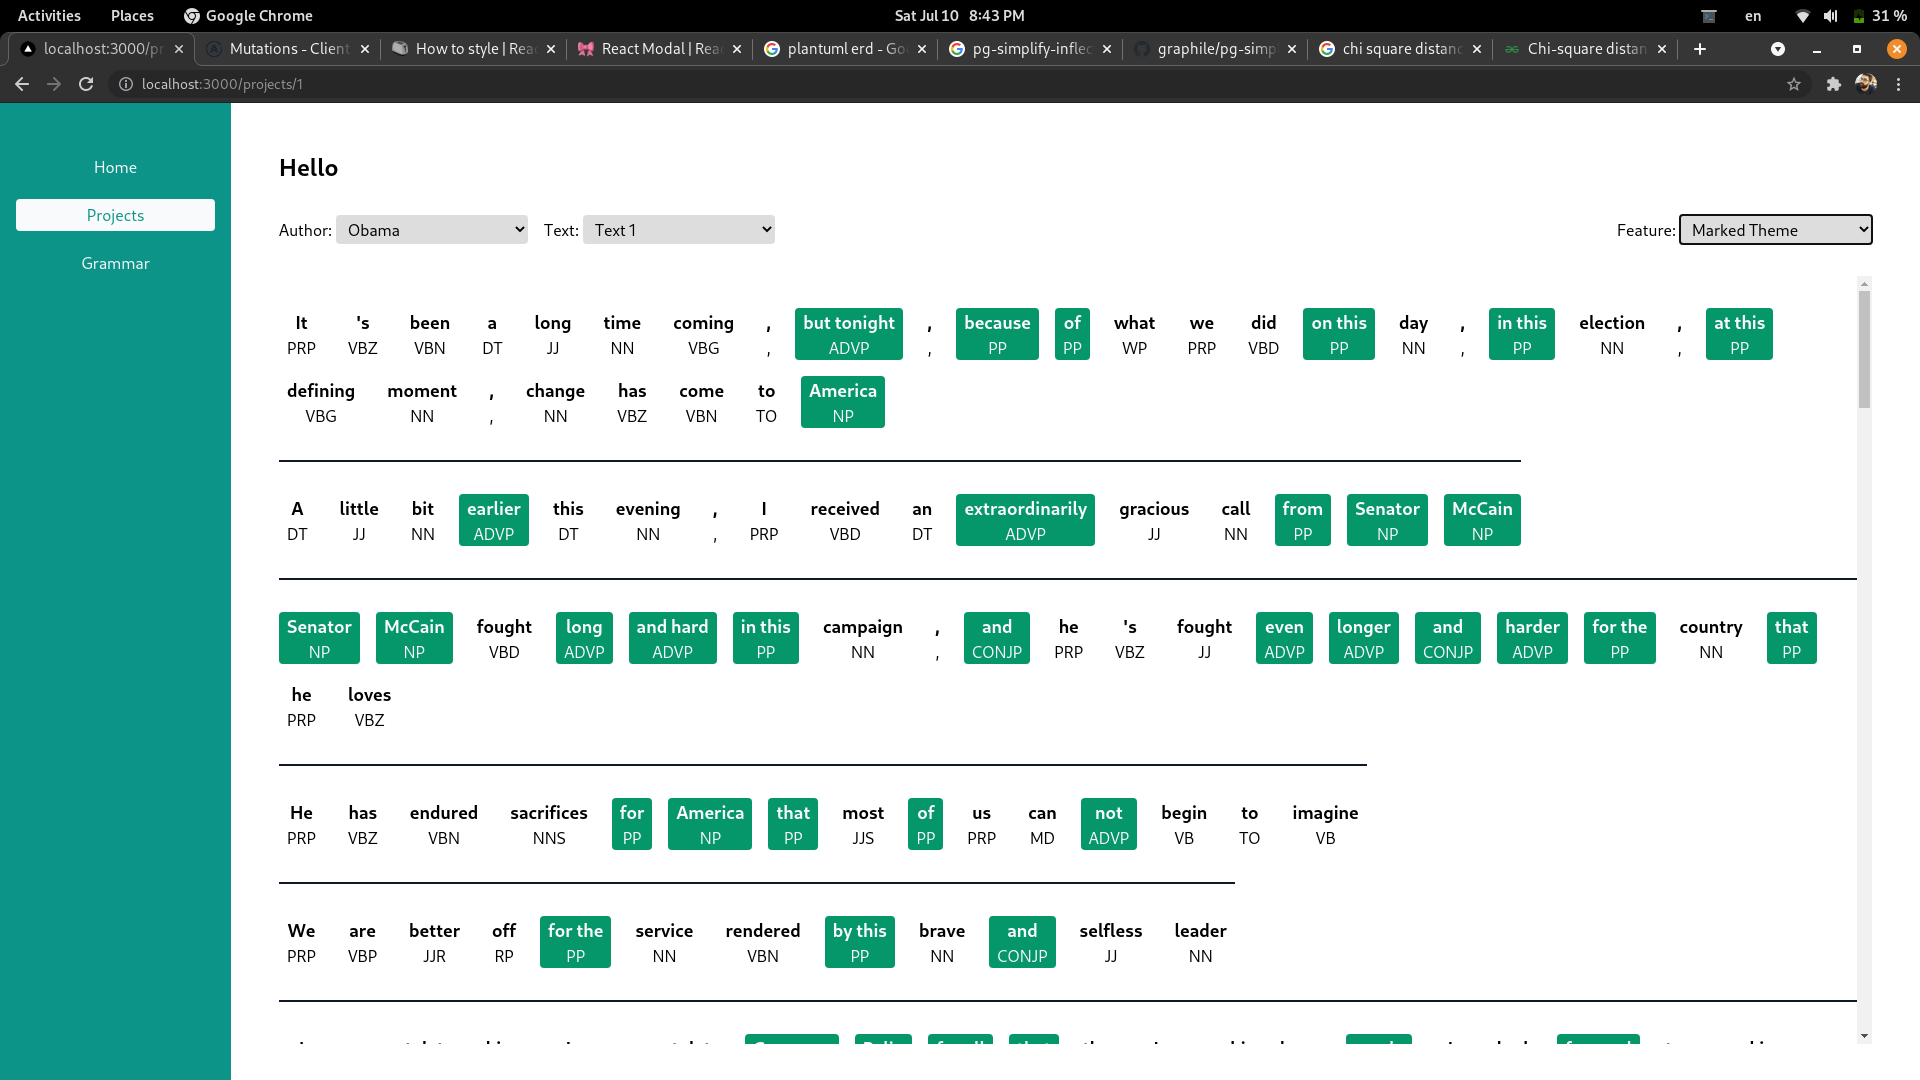
\includegraphics[width=15cm]{images/Project.png}
    \caption{Project}
\end{figure}

\begin{figure}[H]
    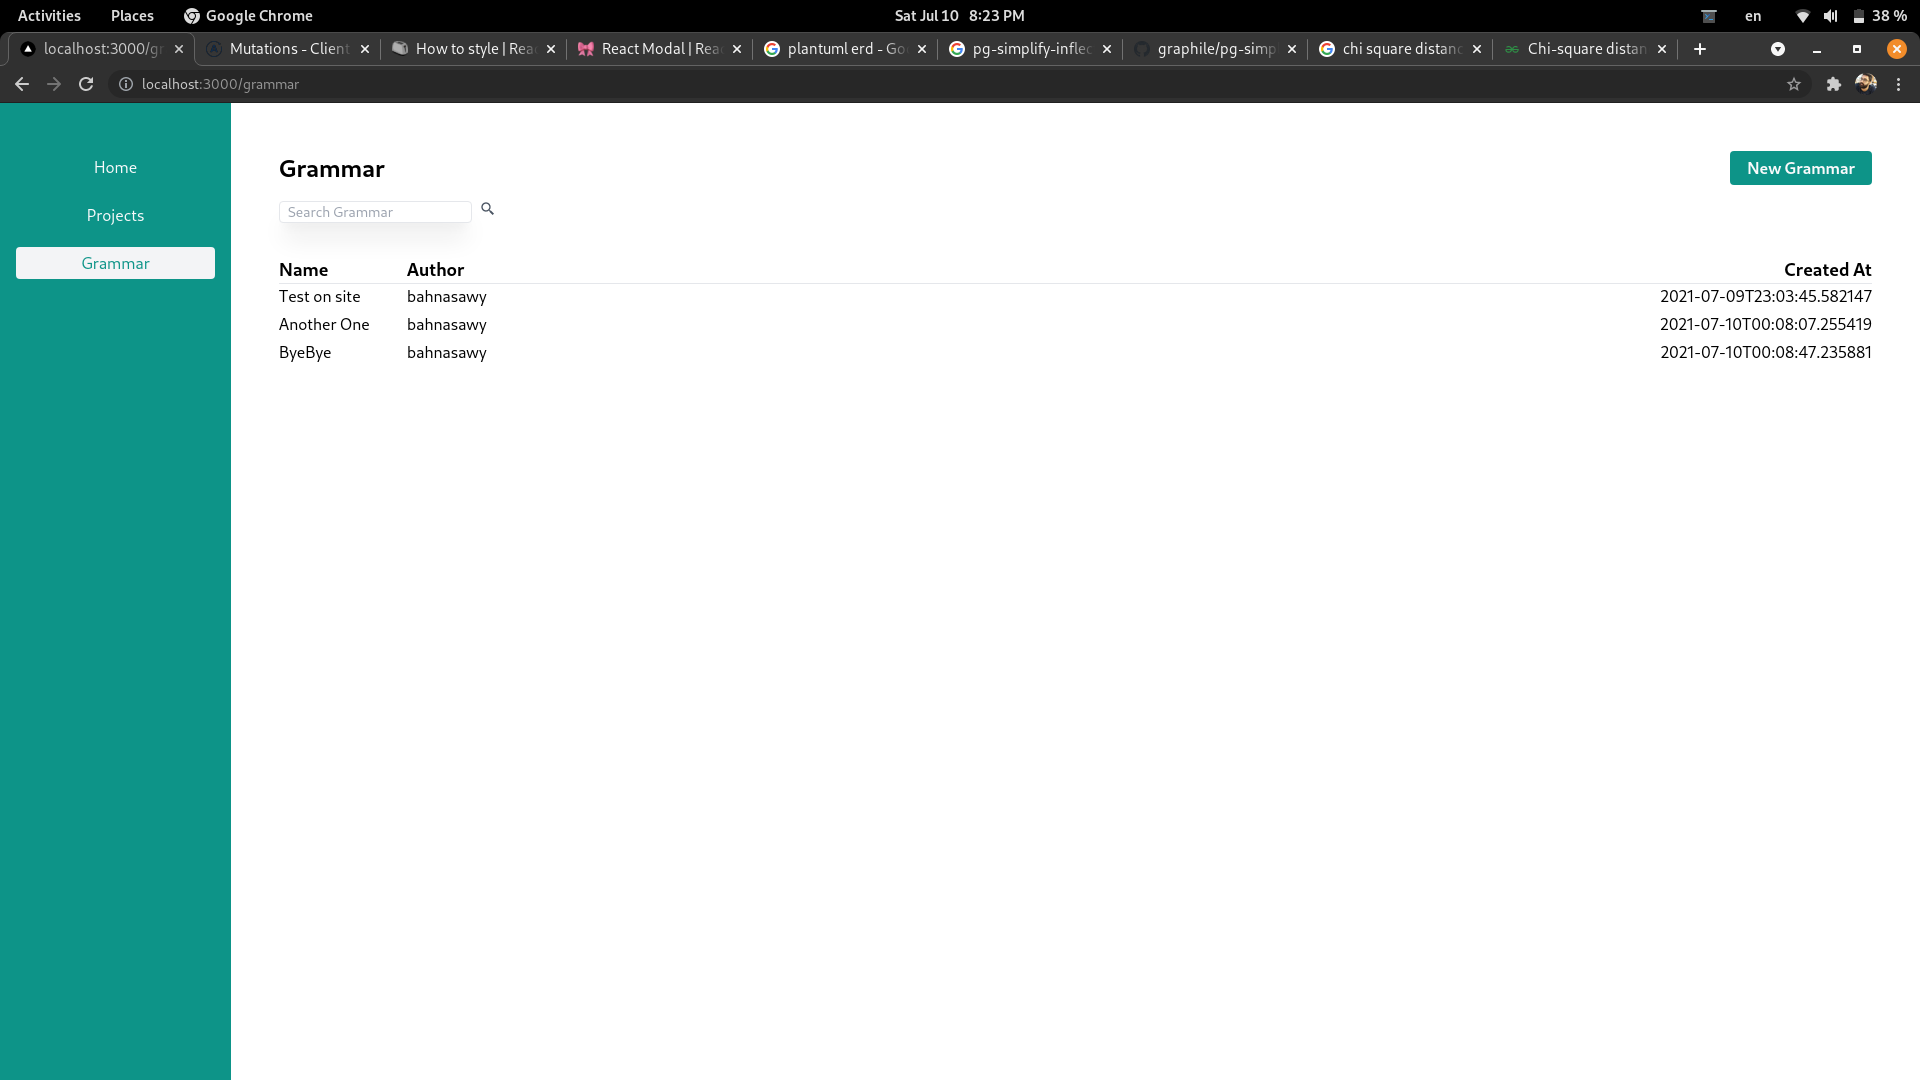
\includegraphics[width=15cm]{images/Grammars.png}
    \caption{Grammars}
\end{figure}

\begin{figure}[H]
    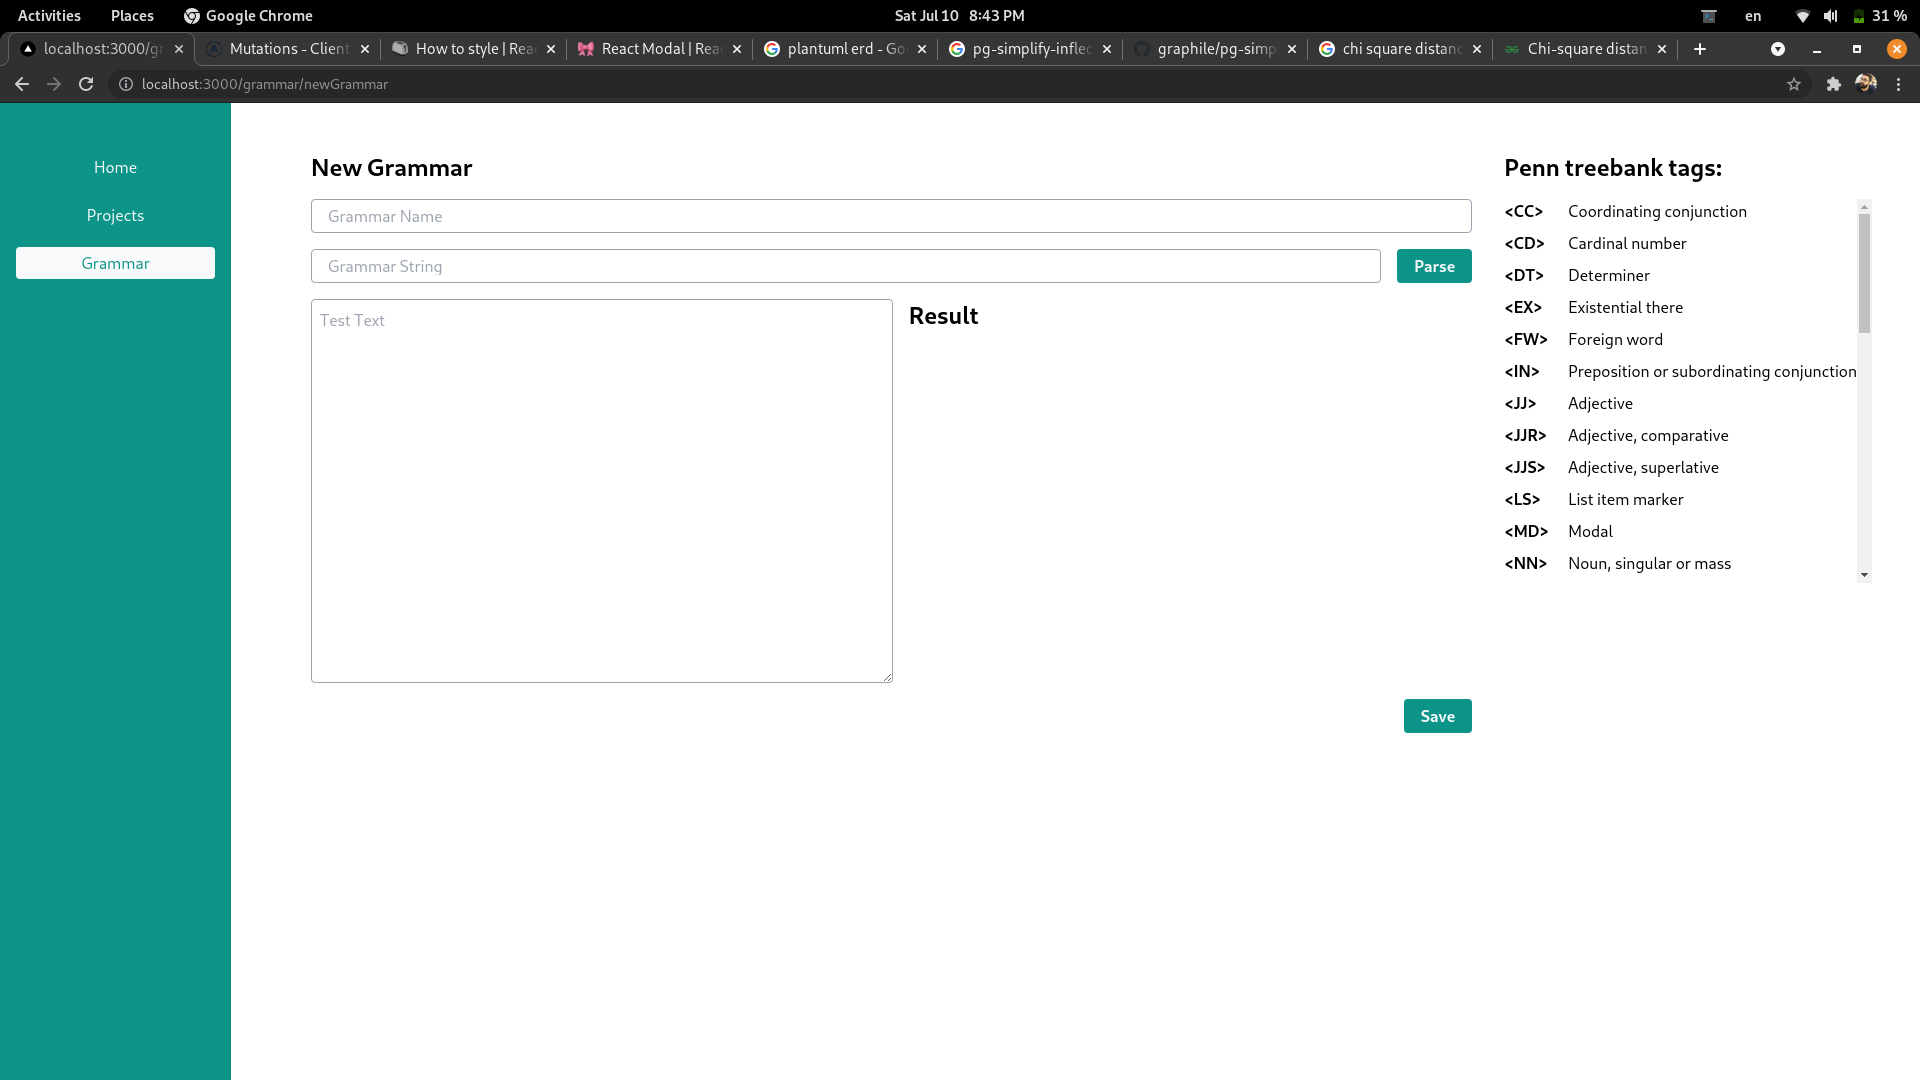
\includegraphics[width=15cm]{images/Grammar.png}
    \caption{Grammar}
\end{figure}

\section{Design Constraints}
No constraints provided.

\section{Other non-functional attributes}
\subsection {Security}
The system will use JWT (JSON Web Token) for user authentication.
\subsection {Reliability}
The system will be deployed as web services on AWS which offers a 99.99\% availability guarantee.
\subsection {Maintainability}
The system will be utilizing the micro-services architecture ensuring smaller and more maintainable code.
\subsection {Portability}
The system will be web based, so it is completely portable.
\subsection {Extensible}
The system is using the micro-services architecture, so it is easily extensible.
\subsection {Re-usability}
The system is using the micro-service architecture, and utilizing the functional programming paradigm, so any bit of code can be reused.

\section{Operational Scenarios}
\begin{figure}[H]
    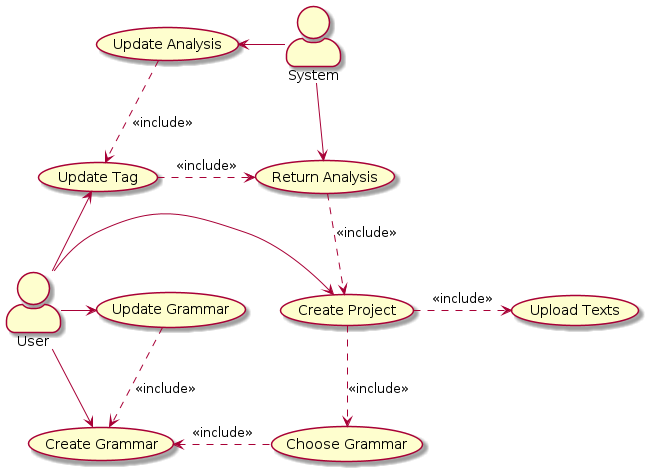
\includegraphics[width=15cm]{images/usecase.png}
    \caption{Use case Diagram}
\end{figure}

\section{Preliminary Schedule Adjusted}
\begin{figure}[H]
    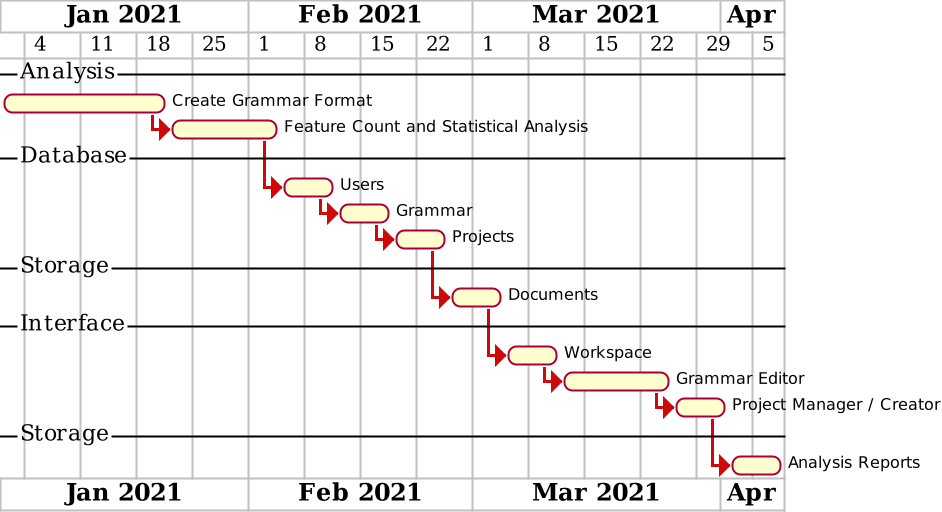
\includegraphics[width=15cm]{images/gantt.png}
    \caption{Gantt Chart}
\end{figure}


